
\chapter{Inleiding}

\section{Routeplanning}

\subsection{Heden}
Routeplanners worden ge�mplementeerd met een API (Application Programming Interface) die al het werk voor zich neemt. Als een cli�nt van plaats X naar Y wil dan berekent de server de korste of snelste weg en geeft het resultaat terug. Om extra features op te vragen, moet de cli�nt parameters meegeven die vermeld staan in de documentatie van de API. Er is dus een sterke koppeling tussen cli�nt en server. Dankzij de opkomst van open data kunnen veel meer features toegevoegd worden aan een routeplanner. Een gebruiker kan bijvoorbeeld kiezen om niet door een regio met een hoog criminaliteitscijfer te reizen. Doordat alleen de server intelligente beslissingen kan nemen, wordt het moeilijk voor de cli�nt om features toe te voegen.

\subsection{Vernieuwing}
Binnen deze masterproef bespreken we een alternatieve methode voor routeplanning. Deze methode maakt gebruik van gelinkte connecties.

Een connectie is simpelweg het vertrek en aankomst van een voertuig. Neem je bijvoorbeeld de trein van station A naar station C en de trein stopt ook in station B, dan bestaat jouw route uit twee connecties: die tussen A en B, B en C. Het kan dus ook zijn dat je moet overstappen in station B.

\begin{figure}[htbp]
   \centering
   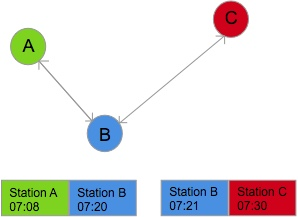
\includegraphics{connectionconcept.jpg} % requires the graphicx package
   \caption{Illustration of the route A - C that exists out of two connections.}
   \label{fig:example}
\end{figure}

Elke route die bestaat dus uit een combinatie van connecties die je via verschillende stations tot je bestemming brengen. 

Deze masterproef onderzoekt hoe connecties van verschillende transportmodi gecombineerd kunnen worden.

\subsection{Voor- en nadelen}
\begin{itemize}
\item Verschillende cli�nts kunnen gemakkelijk gemaakt worden. 
\item Algoritmes die rekening houden met verschillende contexten, bv. rolstoeltoegankelijkheid.
\item Interoperabiliteit van verschillende transitmodi is een Linked Data probleem. Hoe andere stops van andere transportmiddelen bereikbaar zijn, wordt later verduidelijkt. 
\item Schaalbaar: een vervoermaatschappij toevoegen maakt het zoeken van een optimale route niet complexer.
\item Performant dankzij caching.
\end{itemize}

\section{Hoe het begon}

\subsection{Open Data}
Mensen hebben nood aan gebruiksvriendelijke apps die correct gegevens tonen in de juiste context. Bij overheidsdiensten of bedrijven waar elke burger de zogenaamde klant is, ligt de rol van apps bouwen minder bij het de instantie zelf.
Meer en meer bedrijven en overheidsinstanties publiceren hun tijdstabellen als open data. Bij transportbedrijven, zoals De Lijn, is dit ook het geval.

\subsection{GTFS}
GTFS staat voor General Transit Feed Specification. Deze specificatie bepaalt hoe de data van de tijdstabellen van vervoersmaatschappijen opgesteld moet worden. Hierdoor ontstaan er interessante mogelijkheden voor routeplanning door deze GTFS feeds te kunnen combineren.
